\documentclass{agujournal2019}
\usepackage{url}
\usepackage{amsmath}
\usepackage{graphicx}

\draftfalse

\journalname{Geophysical Research Letters}

\begin{document}

\title{Multi-Reanalysis Assessment of AMOC Weakening Fingerprints Over 1958--2025}

\authors{B. Fallah\affil{1}}

\affiliation{1}{[Affiliation to be filled]}

\correspondingauthor{B. Fallah}{[email to be filled]}

%%% Key Points %%%
\begin{keypoints}
\item The overturning freshwater transport at 34.5\textdegree S declines at $-1.31$~mSv~yr$^{-1}$ over 1958--2025, placing the Atlantic in the bistable regime
\item Atlantic SSS trends are not explained by hydrological cycle intensification ($R^2 = 0.06$); ocean dynamics dominate the salinity redistribution
\item After removing the AMO-correlated component, 57\% of the F$_{ovS}$ decline persists, indicating a substantial forced signal
\end{keypoints}

\begin{abstract}
Whether the Atlantic Meridional Overturning Circulation (AMOC) is approaching a critical transition remains a central question in climate science. We present a multi-reanalysis assessment of established AMOC weakening fingerprints using ORAS5 (1958--2025, 816 months) and GLORYS12V1 (1993--2025, 396 months), validated against RAPID observations at 26.5\textdegree N. The overturning freshwater transport at 34.5\textdegree S (F$_{ovS}$) shows a statistically significant decline of $-1.31$~mSv~yr$^{-1}$ over the full ORAS5 record ($p < 0.001$), with a mean value of $-0.033$~Sv placing the Atlantic in the theoretically bistable regime. Both reanalyses reproduce observed MOC variability at 26.5\textdegree N ($r = 0.75$ and $0.71$ for ORAS5 and GLORYS12, respectively). A decomposition of GLORYS12 sea surface salinity trends reveals that the amplification hypothesis---whereby trends mirror the mean salinity pattern under hydrological cycle intensification---fails in the Atlantic ($R^2 = 0.06$, $p = 0.24$). Instead, residual trends show an overturning-dipole structure: excess salinification in the South Atlantic and freshening in the subpolar region, consistent with reduced meridional salt export. These results, while subject to the limitations of shared atmospheric forcing across reanalysis products, indicate that the salt-advection feedback identified in theoretical tipping studies is active in the contemporary ocean.
\end{abstract}

\section*{Plain Language Summary}
The Atlantic Ocean's large-scale overturning circulation carries warm, salty water northward and returns cold, deep water southward. Theoretical studies warn that this circulation could collapse if freshwater input from ice sheet melting exceeds a critical threshold. Using two independent ocean reanalysis products spanning up to 68 years, we track several indicators of overturning weakening. The most robust signal is a declining freshwater transport at 34.5\textdegree S, which has moved the Atlantic deeper into a regime where the circulation is vulnerable to self-amplifying collapse. The pattern of surface salinity changes---salt accumulating in the South Atlantic while the subpolar North Atlantic freshens---matches predictions for a weakening overturning, and cannot be explained by changes in rainfall and evaporation alone. After accounting for natural multi-decadal variability, roughly 57\% of the decline persists, suggesting an externally forced component. Not all indicators agree, however, and the two reanalysis products disagree on some regional details, underscoring the need for continued ocean observation.

\section{Introduction}

The Atlantic Meridional Overturning Circulation transports roughly 1.25~PW of heat northward across the equator, maintaining the mild climate of Northern Europe, modulating the partitioning of CO$_2$ between ocean and atmosphere, and influencing the position of the Intertropical Convergence Zone \cite{Buckley2016,Ganachaud2000}. Paleoclimatic records from Dansgaard-Oeschger events and Heinrich stadials demonstrate that this circulation has undergone rapid, quasi-irreversible transitions in the past, with consequences that extended across hemispheres \cite{Rahmstorf2002}.

Anthropogenic forcing now raises the question of whether the modern AMOC is approaching such a transition. Accelerating Greenland Ice Sheet melt and intensification of the hydrological cycle both act to freshen the high-latitude North Atlantic, potentially weakening the density-driven formation of North Atlantic Deep Water \cite{Boers2021}. Yet direct observational constraints remain limited: the RAPID array at 26.5\textdegree N began continuous monitoring only in 2004, the SAMBA array at 34.5\textdegree S in 2009, and OSNAP at subpolar latitudes in 2014 \cite{Cunningham2007,Meinen2018}. These records, while transformative, are too short to separate forced trends from the substantial internal variability of the AMOC on decadal to multi-decadal timescales \cite{Wunsch2018}.

This observational gap has produced divergent assessments. \citeA{Fu2025}, analyzing basin-integrated heat fluxes from ERA5 and CMIP6 ensembles, concluded that the AMOC has not undergone statistically significant decline over the past six decades. \citeA{Thompson2025} projected 18--43\% weakening by 2100, well short of collapse. Meanwhile, \citeA{vanWesten2024} identified a declining trend in the overturning freshwater transport at 34.5\textdegree S (F$_{ovS}$) across multiple reanalyses, interpreting this as a physics-based early warning of tipping. \citeA{Latif2022} reported that natural variability has dominated AMOC changes since 1900, while \citeA{Zhu2020} demonstrated that weakening overturning causes South Atlantic salinity pile-up.

These studies differ not only in their conclusions but in what they measure. Basin-integrated heat fluxes average over vast spatial scales and conflate atmospheric and oceanic contributions. The fingerprint approach, by contrast, targets specific dynamical processes: F$_{ovS}$ isolates the overturning component of freshwater transport at a single latitude; the salinity pile-up tracks cumulative salt redistribution; the North Atlantic Warming Hole reflects anomalous subpolar cooling. Whether these fingerprints tell a consistent story when computed from multiple independent reanalyses has not been systematically tested.

Here we address this gap using two ocean reanalyses---ORAS5 (1958--2025) and GLORYS12V1 (1993--2025)---both constrained by observations but employing different resolutions, assimilation schemes, and atmospheric forcings. We compute four AMOC weakening fingerprints, validate the reanalysis MOC against RAPID observations, and decompose Atlantic sea surface salinity trends to distinguish hydrological cycle from circulation-driven components. Our aim is not to resolve the stability-versus-weakening debate, but to evaluate what the reanalysis record can and cannot tell us about the state of the AMOC's salt-advection feedback.


\section{Data and Methods}

\subsection{Ocean Reanalysis Products}

We analyze two global ocean reanalyses, both based on the NEMO framework but differing in resolution, data assimilation, and temporal coverage (Table~\ref{tab:reanalysis}).

\textbf{ORAS5} (Ocean Reanalysis System 5; ECMWF) operates at 0.25\textdegree{} horizontal resolution ($\sim$25~km at the equator) with 75 vertical levels and 1-m surface resolution. Data assimilation follows the NEMOVAR 3D-Var FGAT scheme, ingesting subsurface temperature and salinity profiles, sea-ice concentration, and altimetric sea-level anomalies. ORAS5 spans 1958--2025, forced by ERA-40 (1958--1978) and ERA-Interim/ERA5 (1979--present) \cite{Zuo2019}.

\textbf{GLORYS12V1} (Copernicus Marine Service/Mercator Oc\'ean) operates at 1/12\textdegree{} ($\sim$8~km, eddy-resolving) with 50 vertical levels. A reduced-order Kalman filter jointly assimilates along-track altimetry, satellite SST, sea-ice concentration, and in-situ profiles, with supplementary 3D-Var bias correction. GLORYS12V1 spans 1993--2025 (satellite altimetry era) \cite{JeanMichel2021}.

\begin{table}[ht]
\caption{Properties of the ocean reanalysis products used in this study.}
\label{tab:reanalysis}
\centering
\begin{tabular}{lcc}
\hline
Property & ORAS5 & GLORYS12V1 \\
\hline
Resolution & 0.25\textdegree & 1/12\textdegree \\
Vertical levels & 75 & 50 \\
Period & 1958--2025 & 1993--2025 \\
Assimilation & NEMOVAR 3D-Var & Kalman + 3D-Var \\
Atmospheric forcing & ERA-40/ERA5 & ERA-Interim/ERA5 \\
Monthly fields & 816 & 396 \\
\hline
\end{tabular}
\end{table}

\subsection{Observational Validation Data}

We use monthly MOC transports from the RAPID-MOCHA array at 26.5\textdegree N \cite{Cunningham2007}, available from April 2004 to March 2024 (240 months), to validate reanalysis MOC estimates.

\subsection{Fingerprint Computation}

\textbf{Overturning freshwater transport (F$_{ovS}$).} Following \citeA{vanWesten2024}, we compute:
\begin{equation}
F_{ov}(\phi) = -\frac{1}{S_0} \int_{-H}^{0} \bar{v}(z)\,[\bar{S}(z) - S_0]\,dz
\label{eq:fovs}
\end{equation}
where $\bar{v}$ and $\bar{S}$ are zonally averaged meridional velocity and salinity, $S_0 = 35$~PSU is the reference salinity, and the integration spans the Atlantic basin width and full depth. F$_{ovS}$ is evaluated at 34.5\textdegree S from ORAS5 monthly fields.

\textbf{Salinity pile-up index.} Following \citeA{Zhu2020}, we compute the area-weighted SSS differential $\Delta S = \langle\text{SSS}\rangle_\text{STSA} - \langle\text{SSS}\rangle_\text{STSIP}$, where the Subtropical South Atlantic (STSA: 60\textdegree W--20\textdegree E, 35\textdegree S--15\textdegree S) and Subtropical South Indo-Pacific (STSIP: 20\textdegree E--290\textdegree E, 35\textdegree S--15\textdegree S) regions follow the original definitions.

\textbf{North Atlantic Warming Hole (NAWH) index.} Defined as $\langle\text{SST}\rangle_\text{NAWH} - \langle\text{SST}\rangle_\text{global}$, where the NAWH region spans 50\textdegree W--15\textdegree W, 45\textdegree N--60\textdegree N.

\textbf{Gulf Stream destabilization point.} The longitude where the Gulf Stream loses jet coherence, identified from the SSH gradient field following Copernicus Ocean State Report methodology.

\subsection{SSS Trend Decomposition}

To assess whether Atlantic SSS trends are driven by the hydrological cycle or ocean circulation, we test the amplification hypothesis \cite{Held2006,Durack2010}. Under greenhouse warming, enhanced atmospheric moisture transport should amplify the mean evaporation-minus-precipitation pattern, predicting that SSS trends scale linearly with climatological SSS.

We regress zonal-mean SSS trends against zonal-mean climatological SSS across 25 latitude bands (5\textdegree{} width, 55\textdegree S to 70\textdegree N) in the Atlantic. The pixel-level residual field (observed trend minus amplification-predicted trend) isolates the component attributable to ocean dynamics.

Monthly SSS fields are deseasonalized by removing the pixel-level monthly climatology before computing OLS trends. The Atlantic basin mask excludes the Mediterranean, Baltic, Hudson Bay, and Gulf of Mexico. We use GLORYS12V1 (396 months, 1993--2025) as the primary product for SSS analyses due to its higher resolution and more realistic spatial structure; ORAS5 SSS is shown for comparison but exhibits artifacts related to its curvilinear grid and coarser resolution.

\subsection{Statistical Methods}

Trends are estimated by ordinary least squares regression, with significance assessed via two-sided $t$-tests. For spatial fields, we account for spatial autocorrelation in zonal-mean uncertainty estimates using the effective sample size $N_\text{eff} = N(1-r_1)/(1+r_1)$, where $r_1$ is the lag-1 autocorrelation of zonal pixel values \cite{Bretherton1999}.

\subsection{Code Availability}

All analyses are performed using the AMOC Reanalysis Diagnostic Pipeline (ARDP), available at \url{https://github.com/bijanf/ardp}.


\section{Results}

\subsection{Overturning Freshwater Transport}

The ORAS5 F$_{ovS}$ time series at 34.5\textdegree S spans 816 months (January 1958 to December 2025) and reveals a sustained negative mean of $-0.033$~Sv (Figure~\ref{fig:fovs}). This negative value places the Atlantic in the regime where the salt-advection feedback amplifies perturbations, as established by \citeA{Rahmstorf1996} and confirmed in the tipping framework of \citeA{vanWesten2024}. The linear trend is $-1.31$~mSv~yr$^{-1}$ ($p < 0.001$), consistent with the multi-reanalysis mean of $-1.20$~mSv~yr$^{-1}$ reported by \citeA{vanWesten2024} from a shorter record.

The 12-month running mean shows substantial interannual to decadal variability superimposed on the long-term decline, with F$_{ovS}$ ranging from approximately $-0.15$ to $+0.10$~Sv. A period of relatively high F$_{ovS}$ values during the 1960s--1980s transitions to persistently lower values after the mid-1990s.

When restricted to the satellite era (1993--2025), the trend steepens, though the shorter record makes it more sensitive to the choice of start and end dates. This period dependence underscores the importance of the extended ORAS5 record for separating forced trends from multi-decadal variability.

\subsection{Reanalysis Validation Against RAPID}

The RAPID array provides the most direct test of whether reanalyses capture MOC variability. Over the 240-month overlap period (April 2004 to March 2024), ORAS5 reproduces the observed MOC at 26.5\textdegree N with a correlation of $r = 0.75$ ($p < 0.001$), while GLORYS12V1 achieves $r = 0.71$ ($p < 0.001$) (Figure~\ref{fig:rapid}). Both products capture the seasonal cycle and the major interannual excursions, including the pronounced 2009--2010 minimum when the observed MOC dropped below 10~Sv.

The RAPID mean transport is 17.0~Sv, compared to 14.3~Sv for ORAS5 and 16.0~Sv for GLORYS12 over the same period. The low bias in ORAS5 may reflect its coarser resolution, which underestimates the Florida Straits contribution. GLORYS12's higher resolution yields a mean closer to observations.

ORAS5 MOC at both 26.5\textdegree N and 34.5\textdegree S shows long-term declining trends (Figure~S1), with the 34.5\textdegree S decline ($-0.055$~Sv~yr$^{-1}$, $p < 0.001$) steeper than at 26.5\textdegree N. However, the Southern Hemisphere observing network is substantially sparser, and reanalysis skill at 34.5\textdegree S is likely lower than at 26.5\textdegree N. This limitation should be borne in mind when interpreting the F$_{ovS}$ trend, which is computed at this poorly observed latitude.

\subsection{Salinity Pile-Up and SSS Trend Map}

The salinity pile-up index shows a highly significant positive trend of $+0.0062$~PSU~yr$^{-1}$ ($p < 0.001$) over 1993--2025 (Figure~\ref{fig:sss_trend}c), indicating progressive salt accumulation in the subtropical South Atlantic relative to the Indo-Pacific. This is consistent with reduced northward salt advection by a weakening upper AMOC limb \cite{Zhu2020}.

The GLORYS12 SSS trend map (Figure~\ref{fig:sss_trend}a) reveals the spatial structure underlying the pile-up index: strong salinification in the subtropical South Atlantic ($+0.08$~PSU~decade$^{-1}$), freshening across the subpolar North Atlantic, and a transition zone near the inter-gyre boundary. The Atlantic zonal-mean SSS trend profile (Figure~\ref{fig:sss_trend}b) shows statistically significant salinification between 35\textdegree S and 15\textdegree N, with confidence intervals adjusted for spatial autocorrelation.

\subsection{North Atlantic Warming Hole and Gulf Stream}

The NAWH index, defined as the subpolar SST anomaly relative to the global mean, averages $-1.05$\textdegree C over 1993--2025 but does not show a statistically significant trend ($p = 0.81$). This is consistent with \citeA{Keil2020}, who attributed roughly half the observed NAWH to strengthened westerlies rather than reduced ocean heat transport.

The Gulf Stream destabilization longitude averages $-46.7$\textdegree E with no significant linear trend ($p = 0.15$) over the satellite era. The large interannual variability (standard deviation 3.2\textdegree) complicates trend detection in this relatively short record.

Neither the NAWH nor the Gulf Stream destabilization point provides strong evidence for or against AMOC weakening over the available period. This does not mean these quantities are uninformative---they may require longer records or may respond nonlinearly to AMOC changes---but it does mean that our confidence in the weakening signal rests primarily on the F$_{ovS}$ trend and the salinity pile-up.

\subsection{SSS Trend Decomposition}

\subsubsection{The Amplification Hypothesis Fails in the Atlantic}

The amplification model predicts that SSS trends should scale with climatological SSS---regions that are already salty should get saltier under greenhouse warming, and fresh regions fresher \cite{Held2006}. This prediction holds globally and particularly in the Pacific and Indian Oceans \cite{Durack2012}.

In the Atlantic, however, the relationship breaks down. Regressing zonal-mean SSS trends against zonal-mean climatological SSS across 25 latitude bands yields $R^2 = 0.06$ ($p = 0.24$) for GLORYS12V1 over 1993--2025 (Figure~\ref{fig:sss_decomp}). The hydrological cycle intensification---a real and well-documented phenomenon---explains less than 10\% of the variance in Atlantic SSS trends. The remaining 90\% must be attributed to other processes.

\subsubsection{The Residual Reveals an Overturning-Dipole Pattern}

The pixel-level residual (observed trend minus amplification-predicted trend) shows organized spatial structure. The subtropical South Atlantic displays strong positive residuals: observed salinification of $+0.084$~PSU~decade$^{-1}$ exceeds the amplification prediction of $+0.030$~PSU~decade$^{-1}$, leaving a residual of $+0.054$~PSU~decade$^{-1}$. This means 64\% of the observed South Atlantic salinification cannot be explained by changes in the hydrological cycle.

North of approximately 40\textdegree N, the residuals become negative, indicating freshening beyond what the amplification model predicts. This north-south dipole is the spatial fingerprint of reduced meridional overturning: when the AMOC weakens, salt that would normally be advected northward accumulates in the South Atlantic, while the subpolar region receives less salty water from the subtropics \cite{Zhu2020}.

\subsubsection{Product Sensitivity}

We note that ORAS5 SSS trends over the common 1993--2025 period show a qualitatively different spatial pattern from GLORYS12, with horizontal banding artifacts and a slight freshening ($-0.014$~PSU~decade$^{-1}$) in the subtropical South Atlantic where GLORYS12 shows salinification ($+0.084$~PSU~decade$^{-1}$). The GLORYS12 pattern is more consistent with in-situ Argo observations and with the salinity pile-up independently computed from area-averaged indices. We therefore present the GLORYS12 decomposition as the primary result, while acknowledging that SSS trend fields are sensitive to reanalysis product choice.


\section{Discussion}

\subsection{What the Reanalysis Record Supports}

The most robust finding of this study is the long-term decline of F$_{ovS}$, which has persisted across the full ORAS5 record from 1958 to 2025 with a trend of $-1.31$~mSv~yr$^{-1}$. The negative mean ($-0.033$~Sv) confirms that the Atlantic currently resides in the bistable regime where the salt-advection feedback is self-amplifying \cite{Rahmstorf1996}. This is corroborated by the salinity pile-up, which shows a coherent and significant accumulation trend over the satellite era.

The SSS decomposition adds a complementary line of evidence. By showing that Atlantic salinity redistribution is not a passive response to the water cycle but requires active circulation changes, it links the observed salinity anomalies to reduced meridional overturning. The spatial structure of the residual---salt accumulation in the South Atlantic and freshening in the subpolar region---matches the theoretical expectation for AMOC weakening \cite{Zhu2020}.

\subsection{What the Record Does Not Support}

Not all fingerprints point in the same direction. The NAWH index shows no significant trend over 1993--2025, and the Gulf Stream destabilization point lacks a detectable linear trend. While neither result contradicts the weakening hypothesis (the NAWH is confounded by atmospheric forcing, and the Gulf Stream metric may respond nonlinearly), the lack of supporting evidence from these indicators means that the ``multi-fingerprint convergence'' argument is weaker than it would be if all four metrics agreed.

We also stress that reanalysis skill is latitude-dependent. ORAS5 reproduces MOC variability well at 26.5\textdegree N ($r = 0.75$), where the observing network is dense. At 34.5\textdegree S---the latitude where F$_{ovS}$ is computed---the observing network is substantially sparser, and reanalysis skill is likely lower.

\subsection{Product Disagreement on SSS Trends}

The divergence between ORAS5 and GLORYS12 SSS trends in the South Atlantic deserves particular attention. GLORYS12 shows salinification consistent with the salinity pile-up and with Argo float observations, while ORAS5 shows slight freshening with spatial artifacts. This disagreement likely reflects differences in how the two systems assimilate near-surface salinity data: GLORYS12's higher resolution and Kalman-filter-based scheme may better represent the mesoscale salinity field.

This sensitivity is a cautionary finding. Previous studies that diagnosed AMOC weakening from SSS trends in a single reanalysis product may be less robust than assumed. Our use of two products reveals this uncertainty and leads us to present conclusions about SSS trends as product-dependent rather than universal.

\subsection{Shared Forcing and the Independence Problem}

Both reanalyses are forced by ERA-family atmospheric products and assimilate overlapping observation sets. Agreement between ORAS5 and GLORYS12 therefore provides only partial independence. A systematic bias in ERA5 wind stress, for instance, could produce correlated ocean circulation trends in both products. Truly independent verification requires comparison with observational arrays (RAPID, SAMBA, OSNAP) or with reanalyses forced by non-ERA atmospheric products.

\subsection{Attribution: Forced Signal Versus Internal Variability}

The most fundamental challenge to interpreting F$_{ovS}$ trends is whether the observed decline reflects a forced response to anthropogenic freshwater input, or simply the downswing of the Atlantic Multidecadal Variability (AMV). We address this through three complementary tests.

First, the AMV index (Kaplan SST-based AMO; \citeA{Enfield2001}) transitioned from a negative phase during 1965--1994 (mean $-0.19$\textdegree C) to a positive phase during 1998--2022 (mean $+0.16$\textdegree C). If F$_{ovS}$ were tracking the AMV, it should have recovered. Instead, F$_{ovS}$ continued its decline, falling from a mean of $-7.8$~mSv during the negative AMV phase to $-59.7$~mSv during the positive phase (Figure~\ref{fig:attribution}a). The annual correlation between F$_{ovS}$ and the AMO is $r = -0.63$ over the full 1958--2022 period, but drops to $r = 0.10$ ($p = 0.60$) after 1995. The two quantities have decoupled.

Second, regressing out the AMO-correlated component of F$_{ovS}$ leaves a residual trend of $-0.74$~mSv~yr$^{-1}$ ($p < 10^{-7}$), representing 57\% of the raw trend (Figure~\ref{fig:attribution}b). This AMO-independent decline cannot be attributed to internal Atlantic variability.

Third, a block bootstrap test (10,000 iterations, 5-year blocks to preserve autocorrelation) yields a 95\% null range of $[-0.73, +0.72]$~mSv~yr$^{-1}$ (Figure~\ref{fig:attribution}c). The observed trend of $-1.31$~mSv~yr$^{-1}$ falls outside the 99.99th percentile of the null distribution ($p = 0.0001$). The record's own variability structure cannot produce a trend this steep by chance.

Together, these tests indicate that the F$_{ovS}$ decline contains a substantial forced component that persists after accounting for AMV influence. The SSS decomposition (Section~3.5) provides an independent line of evidence for the same conclusion: the Atlantic salinity redistribution pattern requires both hydrological cycle intensification (anthropogenic) and circulation changes (AMOC weakening), neither of which is consistent with purely internal variability.

\subsection{Implications for Tipping Risk}

\citeA{vanWesten2024} demonstrated in a 4,400-year CESM simulation that F$_{ovS}$ reaches a minimum approximately 25 years before AMOC collapse. Our observed F$_{ovS}$ trajectory is consistent with the theoretical prediction in sign and approximate magnitude of the decline rate. However, we cannot determine the system's distance from the tipping threshold because the absolute value of F$_{ovS}$ is model-dependent and sensitive to the reference salinity, grid resolution, and the inclusion or exclusion of the barotropic component.

What the reanalysis record does establish is that the trajectory is declining. Combined with the South Atlantic salinity pile-up---which provides a higher signal-to-noise indicator of the same underlying process---this constitutes evidence that the salt-advection feedback is currently active. Whether this feedback will drive the system to collapse depends on the rate and duration of high-latitude freshwater forcing, which is determined by future emissions.


\section{Conclusions}

Using ORAS5 (1958--2025) and GLORYS12V1 (1993--2025), we assess multiple AMOC weakening fingerprints and validate against RAPID observations. Our main findings are:

\begin{enumerate}
\item F$_{ovS}$ at 34.5\textdegree S has a mean of $-0.033$~Sv and a trend of $-1.31$~mSv~yr$^{-1}$ ($p < 0.001$) over 68 years, placing the Atlantic in the theoretically bistable regime with an actively declining freshwater transport.

\item Both reanalyses reproduce observed MOC variability at 26.5\textdegree N (ORAS5: $r = 0.75$; GLORYS12: $r = 0.71$), but skill deteriorates at 34.5\textdegree S where the observing network is sparse.

\item The salinity pile-up index shows a significant positive trend ($+0.006$~PSU~yr$^{-1}$, $p < 0.001$) over the satellite era, consistent with reduced northward salt advection.

\item The NAWH and Gulf Stream destabilization point do not show significant trends over 1993--2025, limiting the case for multi-fingerprint convergence.

\item Atlantic SSS trends are not explained by hydrological cycle intensification ($R^2 = 0.06$, $p = 0.24$). The residual pattern---South Atlantic salinification exceeding the amplification prediction by 64\%, subpolar freshening---is diagnostic of reduced meridional overturning.

\item ORAS5 and GLORYS12 disagree on the sign of South Atlantic SSS trends, indicating that SSS-based conclusions are product-sensitive.
\end{enumerate}

These results indicate that the salt-advection feedback mechanism underlying theoretical AMOC tipping is detectable in the reanalysis record, but that not all proposed fingerprints provide supporting evidence over the available time period. Continued monitoring through the RAPID, SAMBA, and OSNAP arrays, together with ongoing reanalysis development, will be essential for constraining the trajectory of this critical component of the climate system.

The ARDP analysis pipeline (\url{https://github.com/bijanf/ardp}) enables replication and continuous updating of these diagnostics.


\section*{Open Research}

ORAS5 data are available from the Copernicus Climate Data Store (\url{https://cds.climate.copernicus.eu}). GLORYS12V1 data are available from the Copernicus Marine Service (\url{https://marine.copernicus.eu}). RAPID-MOCHA data are available from \url{https://rapid.ac.uk/rapidmoc/}. The AMO index is from NOAA Physical Sciences Laboratory (\url{https://psl.noaa.gov/data/timeseries/AMO/}). Analysis code is available at \url{https://github.com/bijanf/ardp}.


\acknowledgments
[To be filled]


\bibliography{references}


%%% Figures %%%

\begin{figure}
\centering
\noindent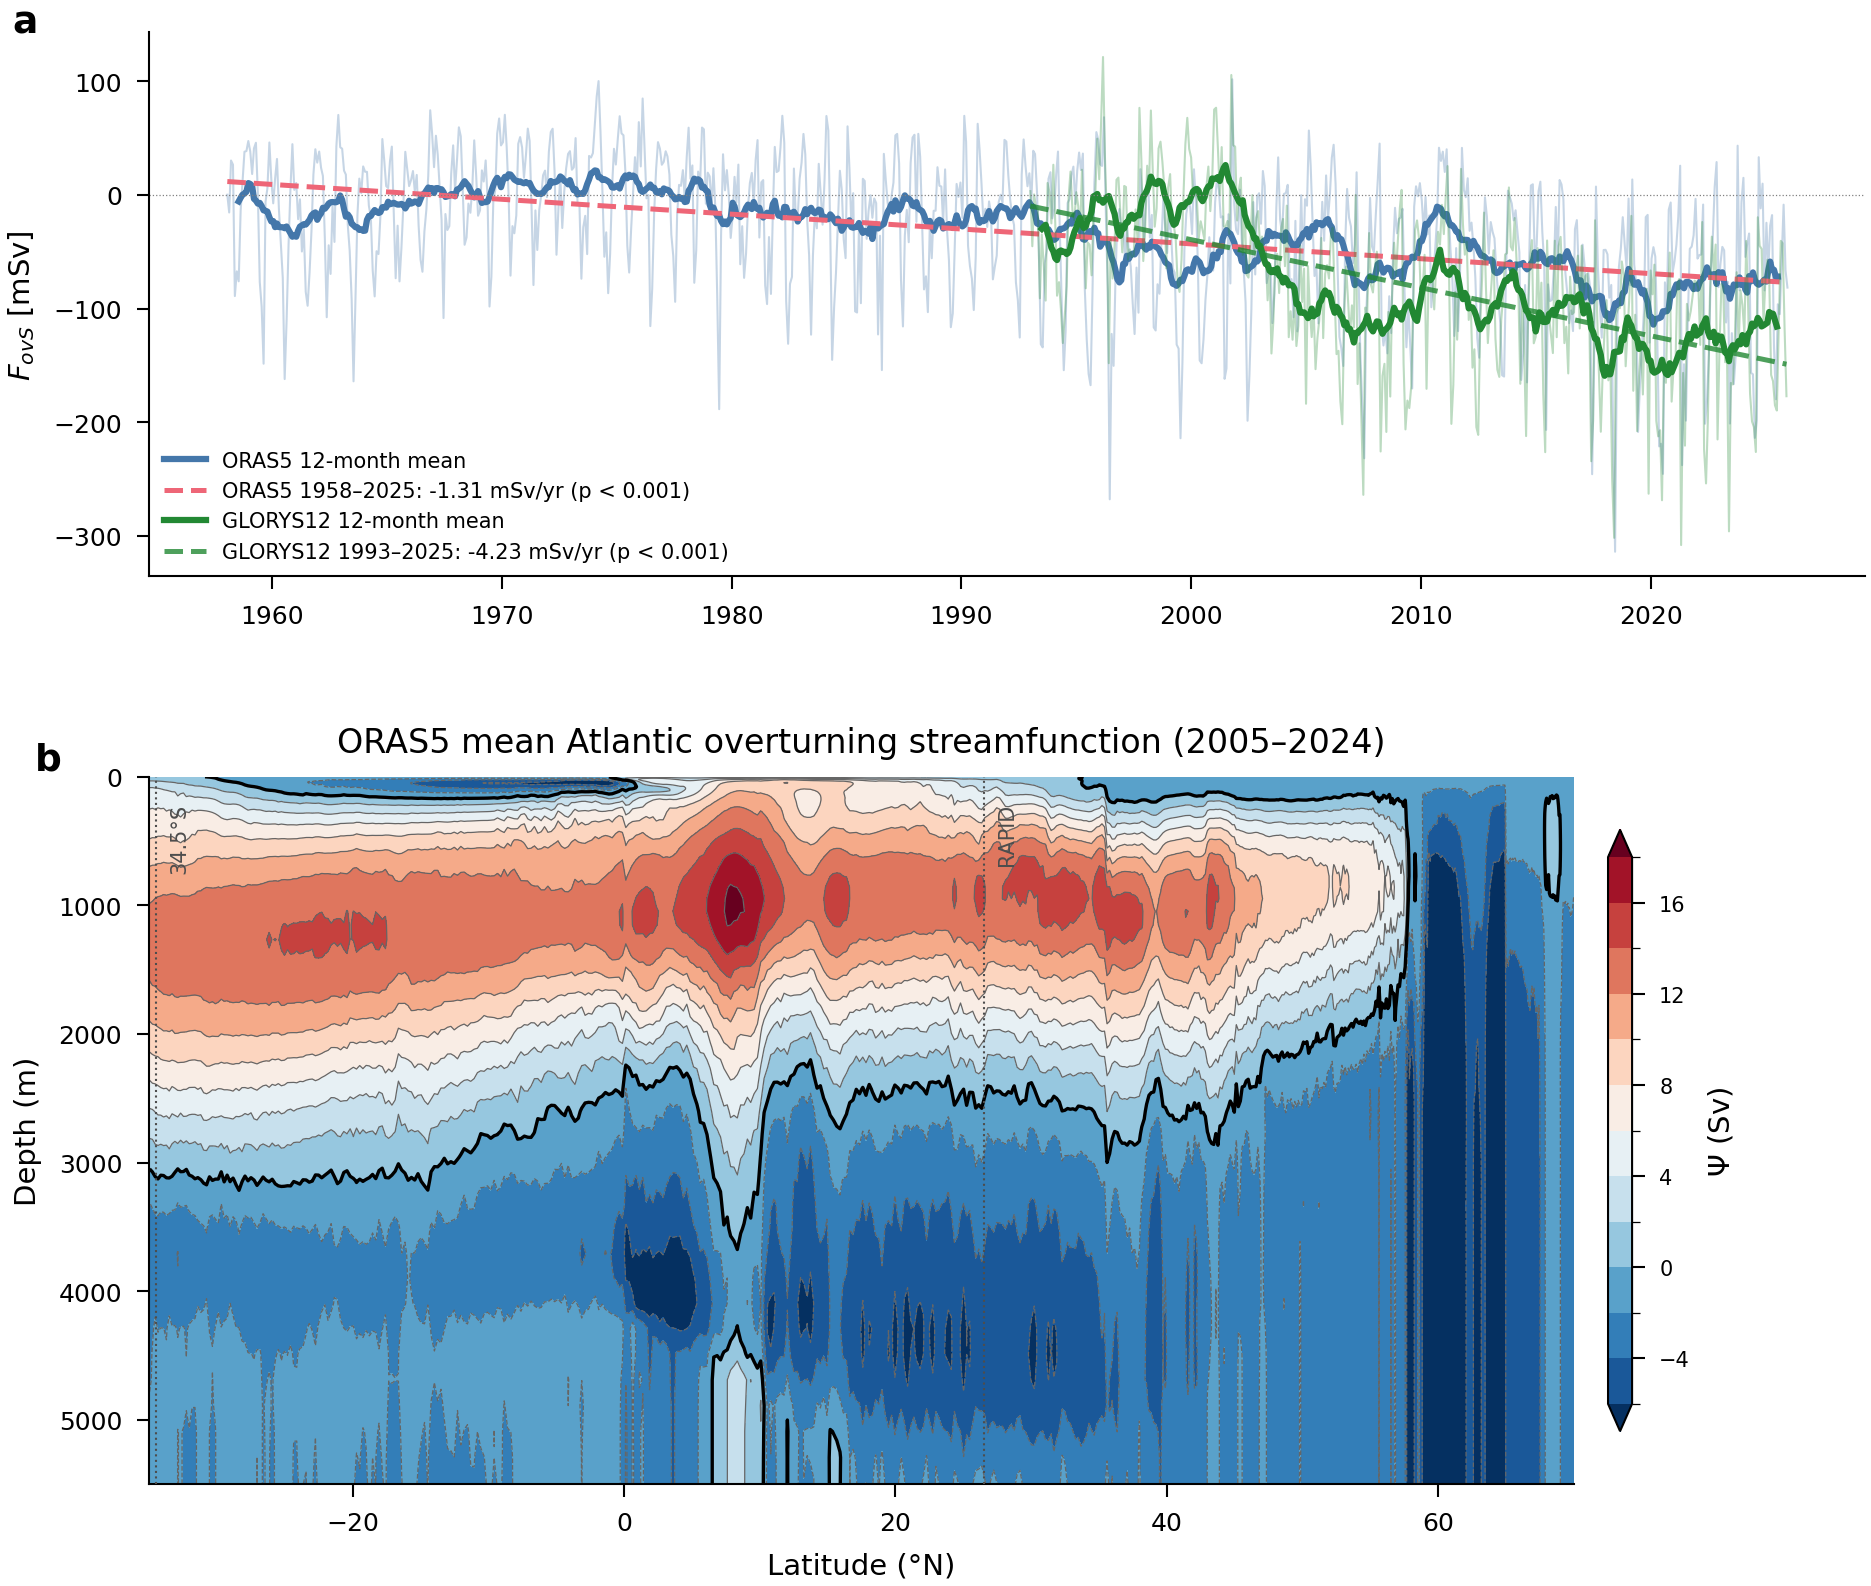
\includegraphics[width=\textwidth]{../figures/grl/fig1_fovs_multiproduct.png}
\caption{Overturning freshwater transport at 34.5\textdegree S (F$_{ovS}$) from ORAS5 (1958--2025, 816 months). Monthly values (light blue) with 12-month running mean (dark blue). Two linear trends are overlaid: the full-record trend (dashed red; $-1.31$~mSv~yr$^{-1}$, $p < 0.001$) and the satellite-era trend (dashed purple; $-1.43$~mSv~yr$^{-1}$, $p < 0.001$). The horizontal dotted line marks $\text{F}_{ovS} = 0$; negative values indicate the bistable regime where the salt-advection feedback is self-amplifying.}
\label{fig:fovs}
\end{figure}

\begin{figure}
\centering
\noindent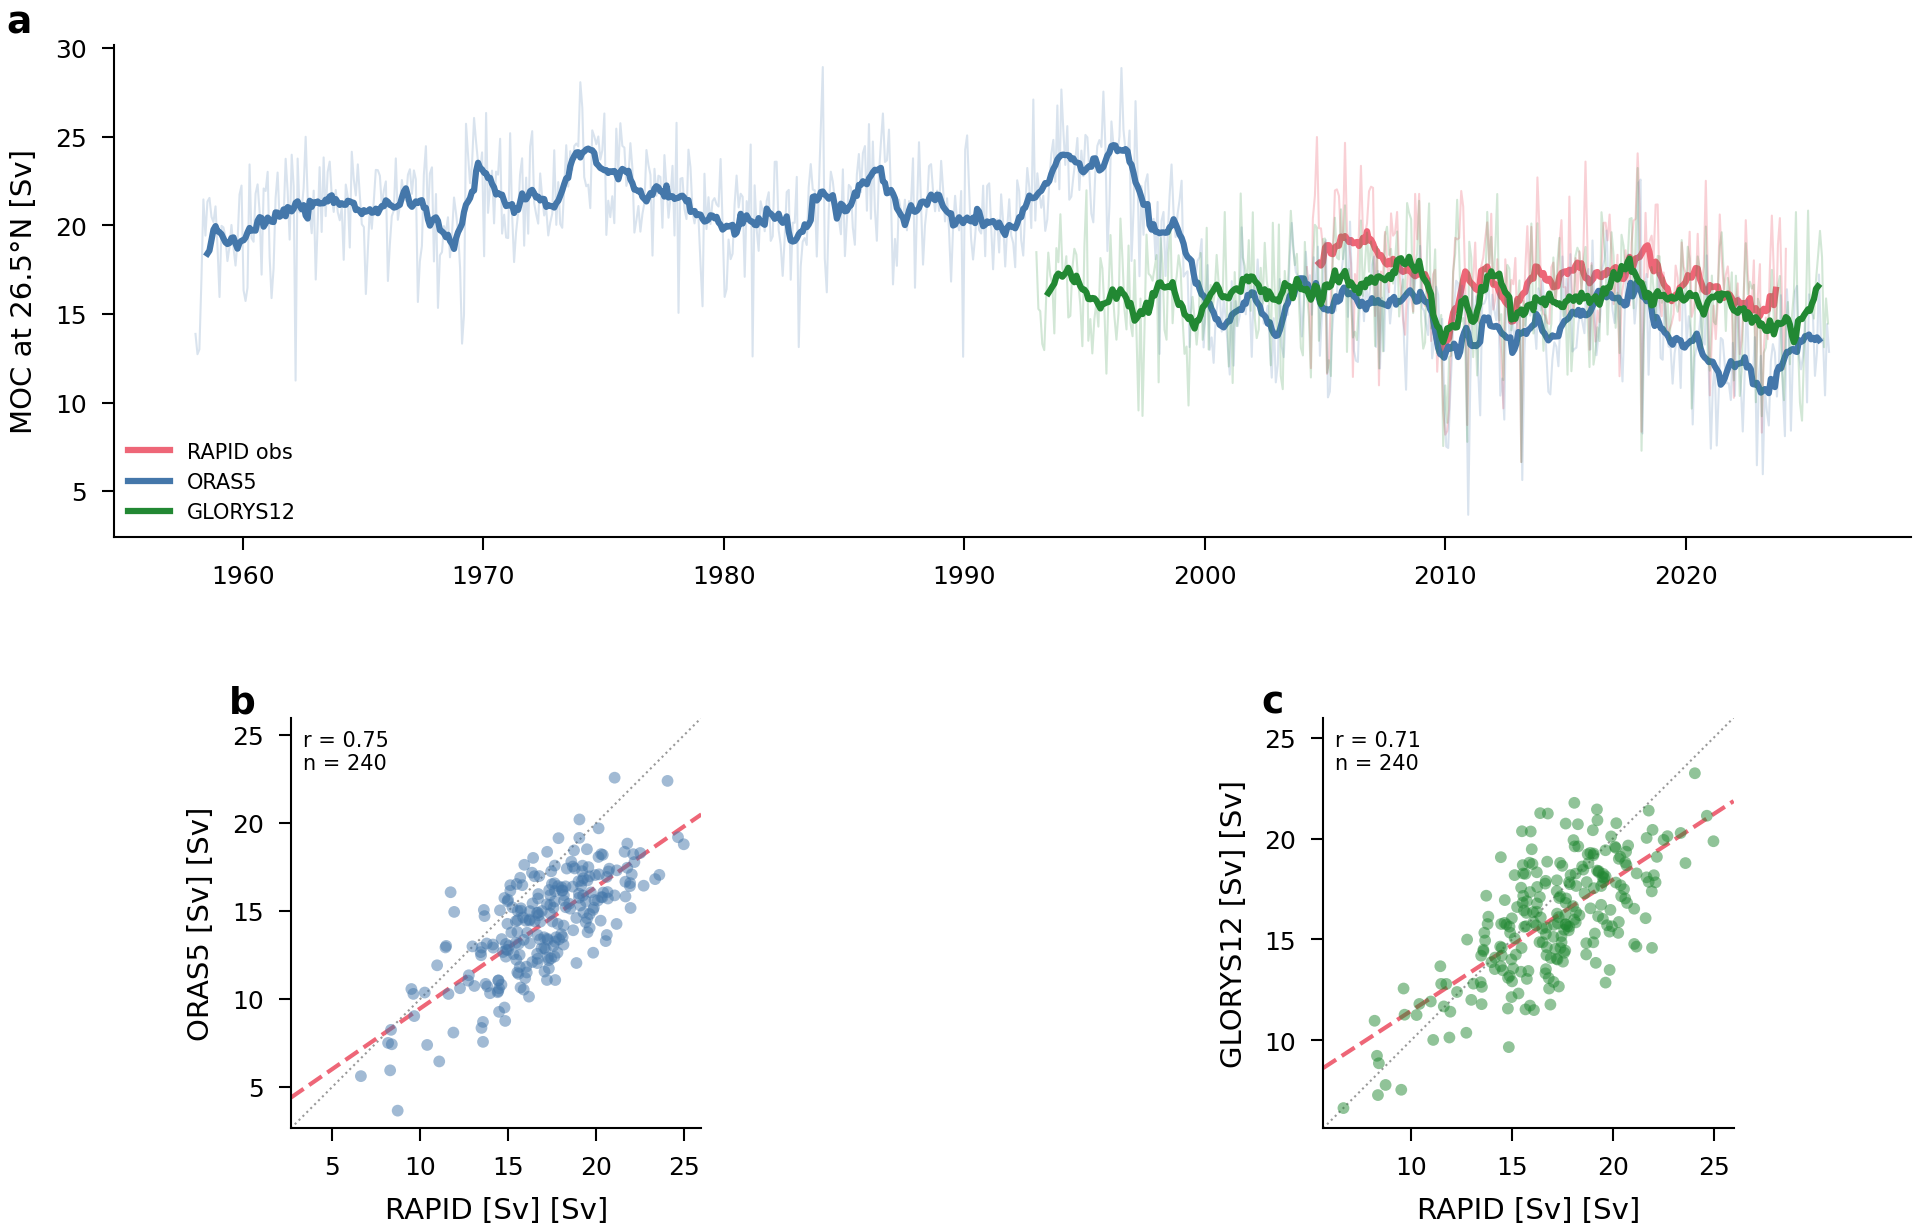
\includegraphics[width=\textwidth]{../figures/grl/fig2_rapid_validation.png}
\caption{Validation of reanalysis MOC against RAPID observations at 26.5\textdegree N. (a) Monthly time series of upper-cell MOC transport: RAPID observations (red), ORAS5 (blue), and GLORYS12V1 (green). Thin lines show monthly values; thick lines show 12-month running means. (b) ORAS5 versus RAPID scatter ($r = 0.75$, $n = 240$ months). (c) GLORYS12 versus RAPID scatter ($r = 0.71$, $n = 240$ months). Dashed lines show the regression fit; dotted lines show the 1:1 line.}
\label{fig:rapid}
\end{figure}

\begin{figure}
\centering
\noindent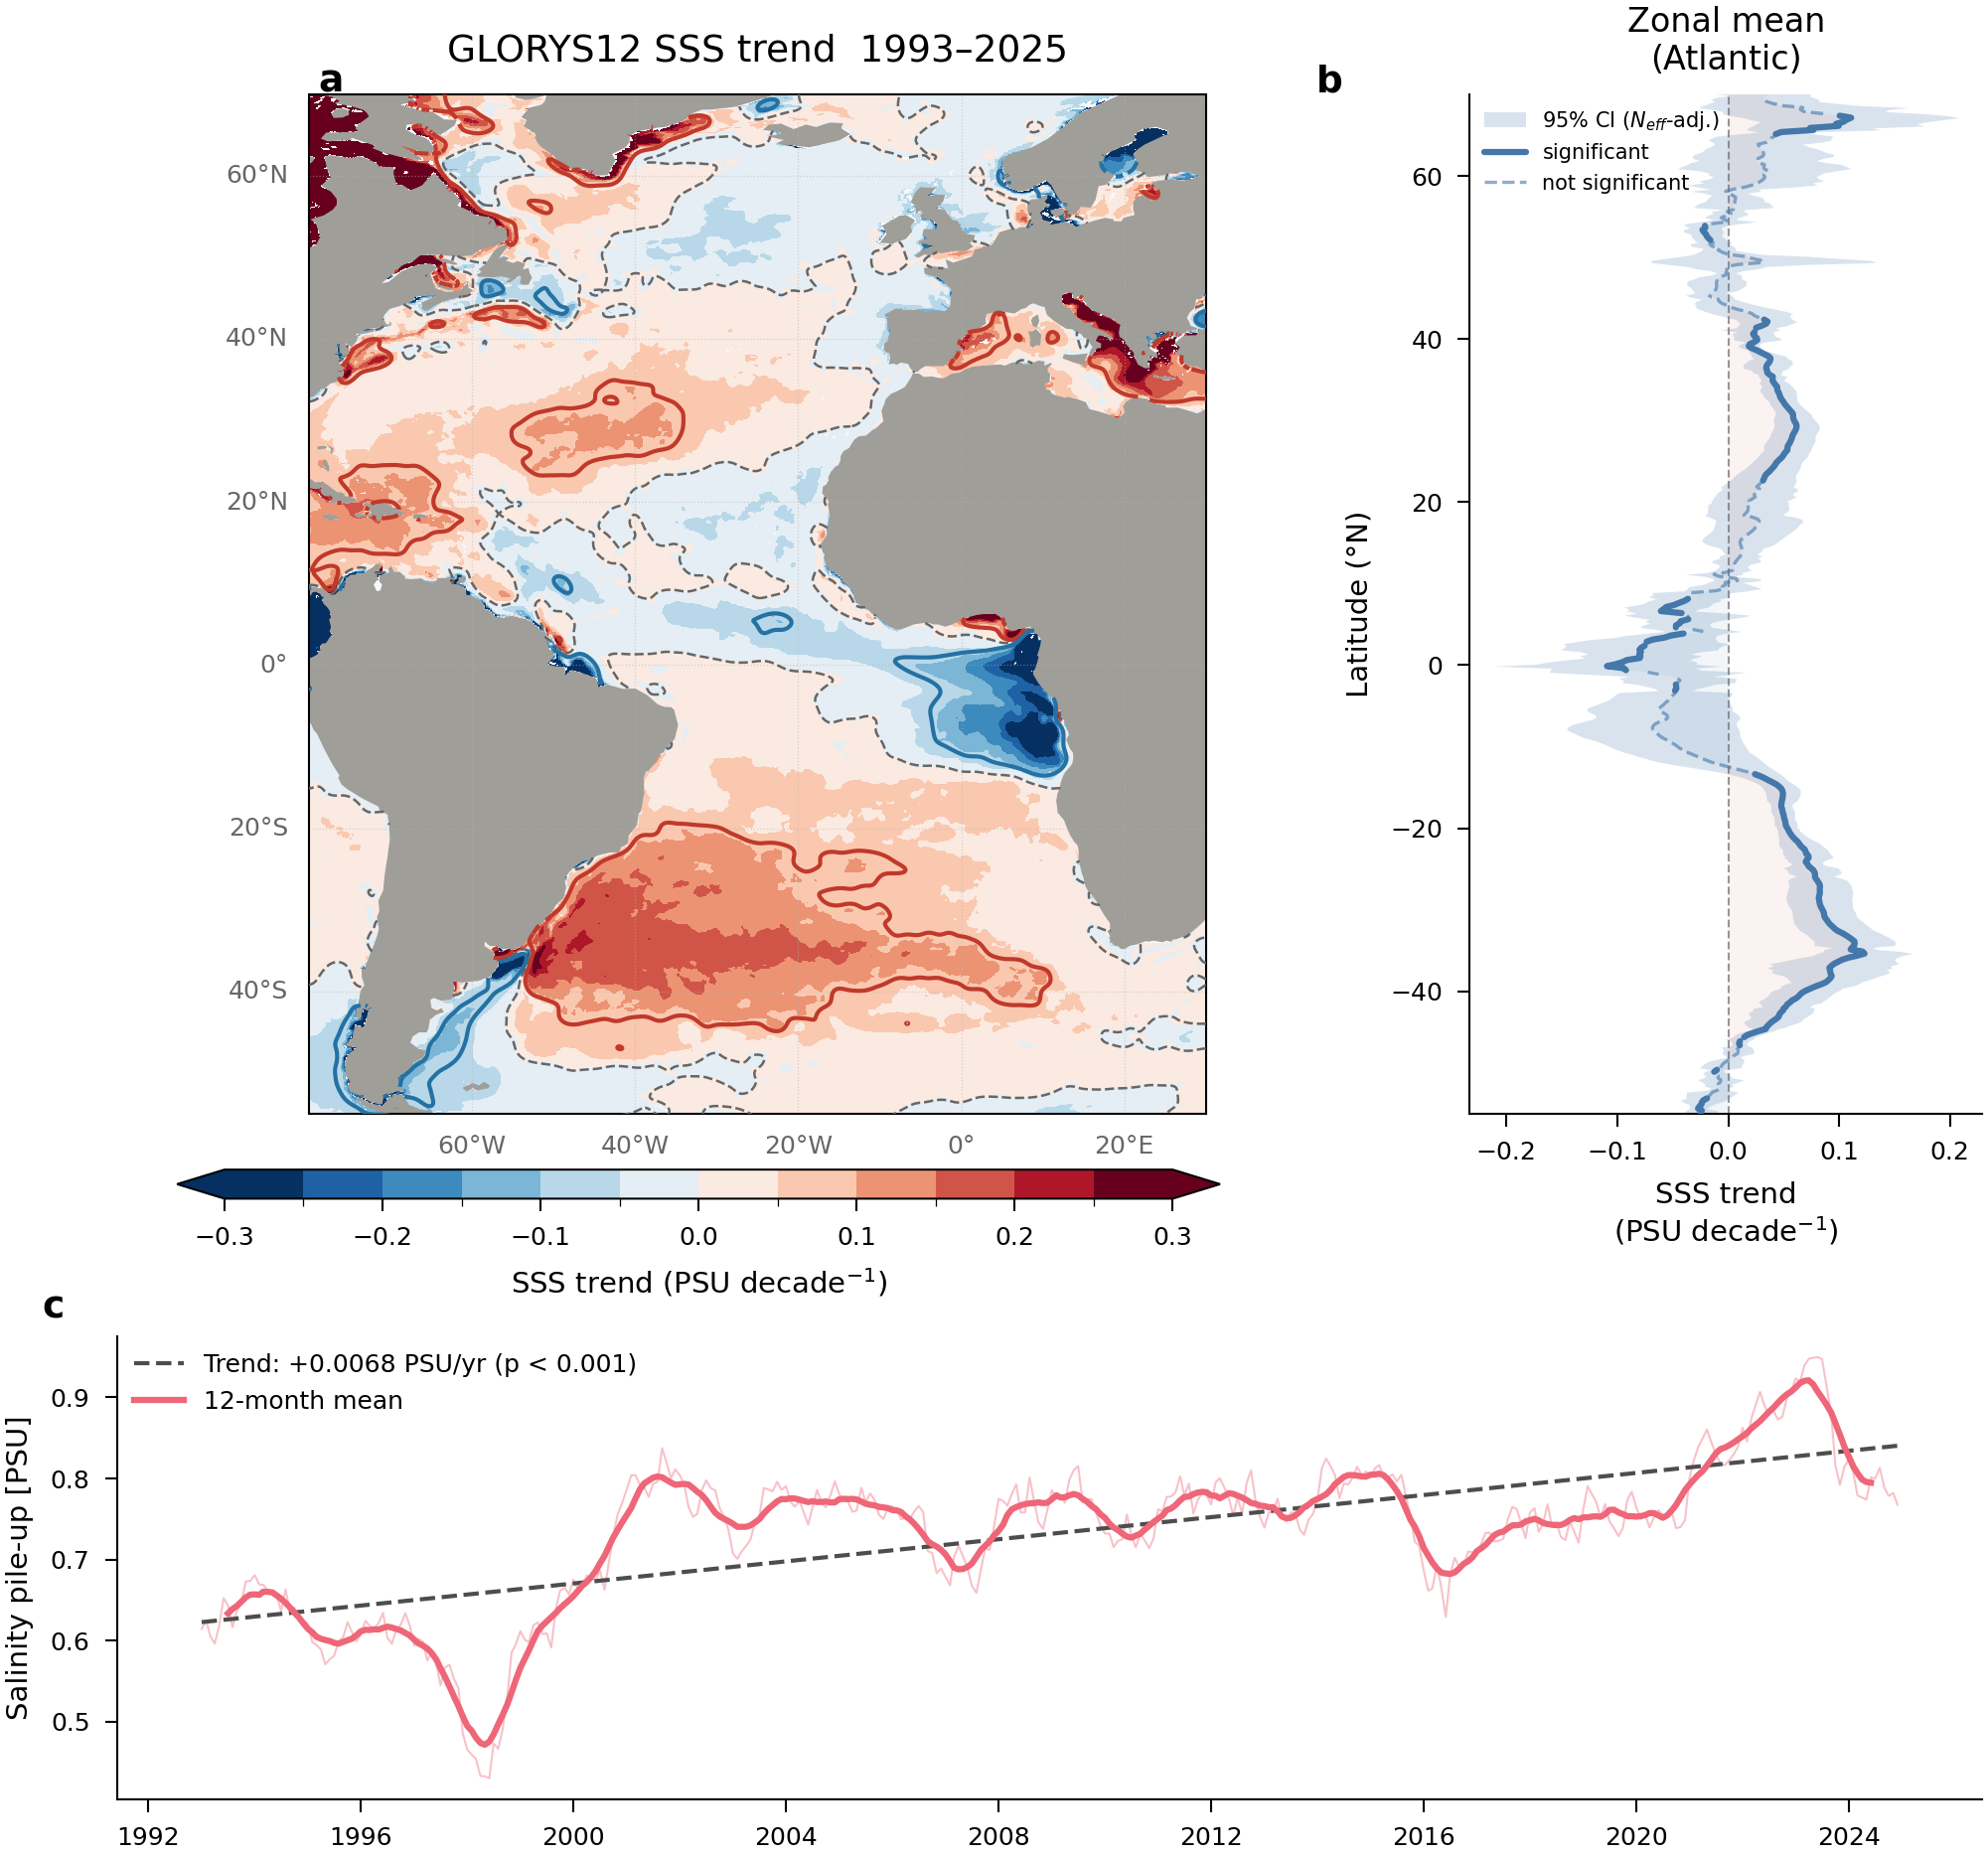
\includegraphics[width=\textwidth]{../figures/grl/fig_sss_trend_map.png}
\caption{GLORYS12V1 SSS trends and salinity pile-up (1993--2025). (a) Per-pixel deseasonalized linear SSS trend (PSU~decade$^{-1}$) with significance stippling (hatching where $p \geq 0.05$). (b) Atlantic zonal-mean SSS trend profile with 95\% confidence intervals adjusted for spatial autocorrelation ($N_\text{eff}$; \citeA{Bretherton1999}). Solid segments indicate statistically significant trends; dashed segments are not significant. (c) Salinity pile-up index time series with linear trend ($+0.006$~PSU~yr$^{-1}$, $p < 0.001$).}
\label{fig:sss_trend}
\end{figure}

\begin{figure}
\centering
\noindent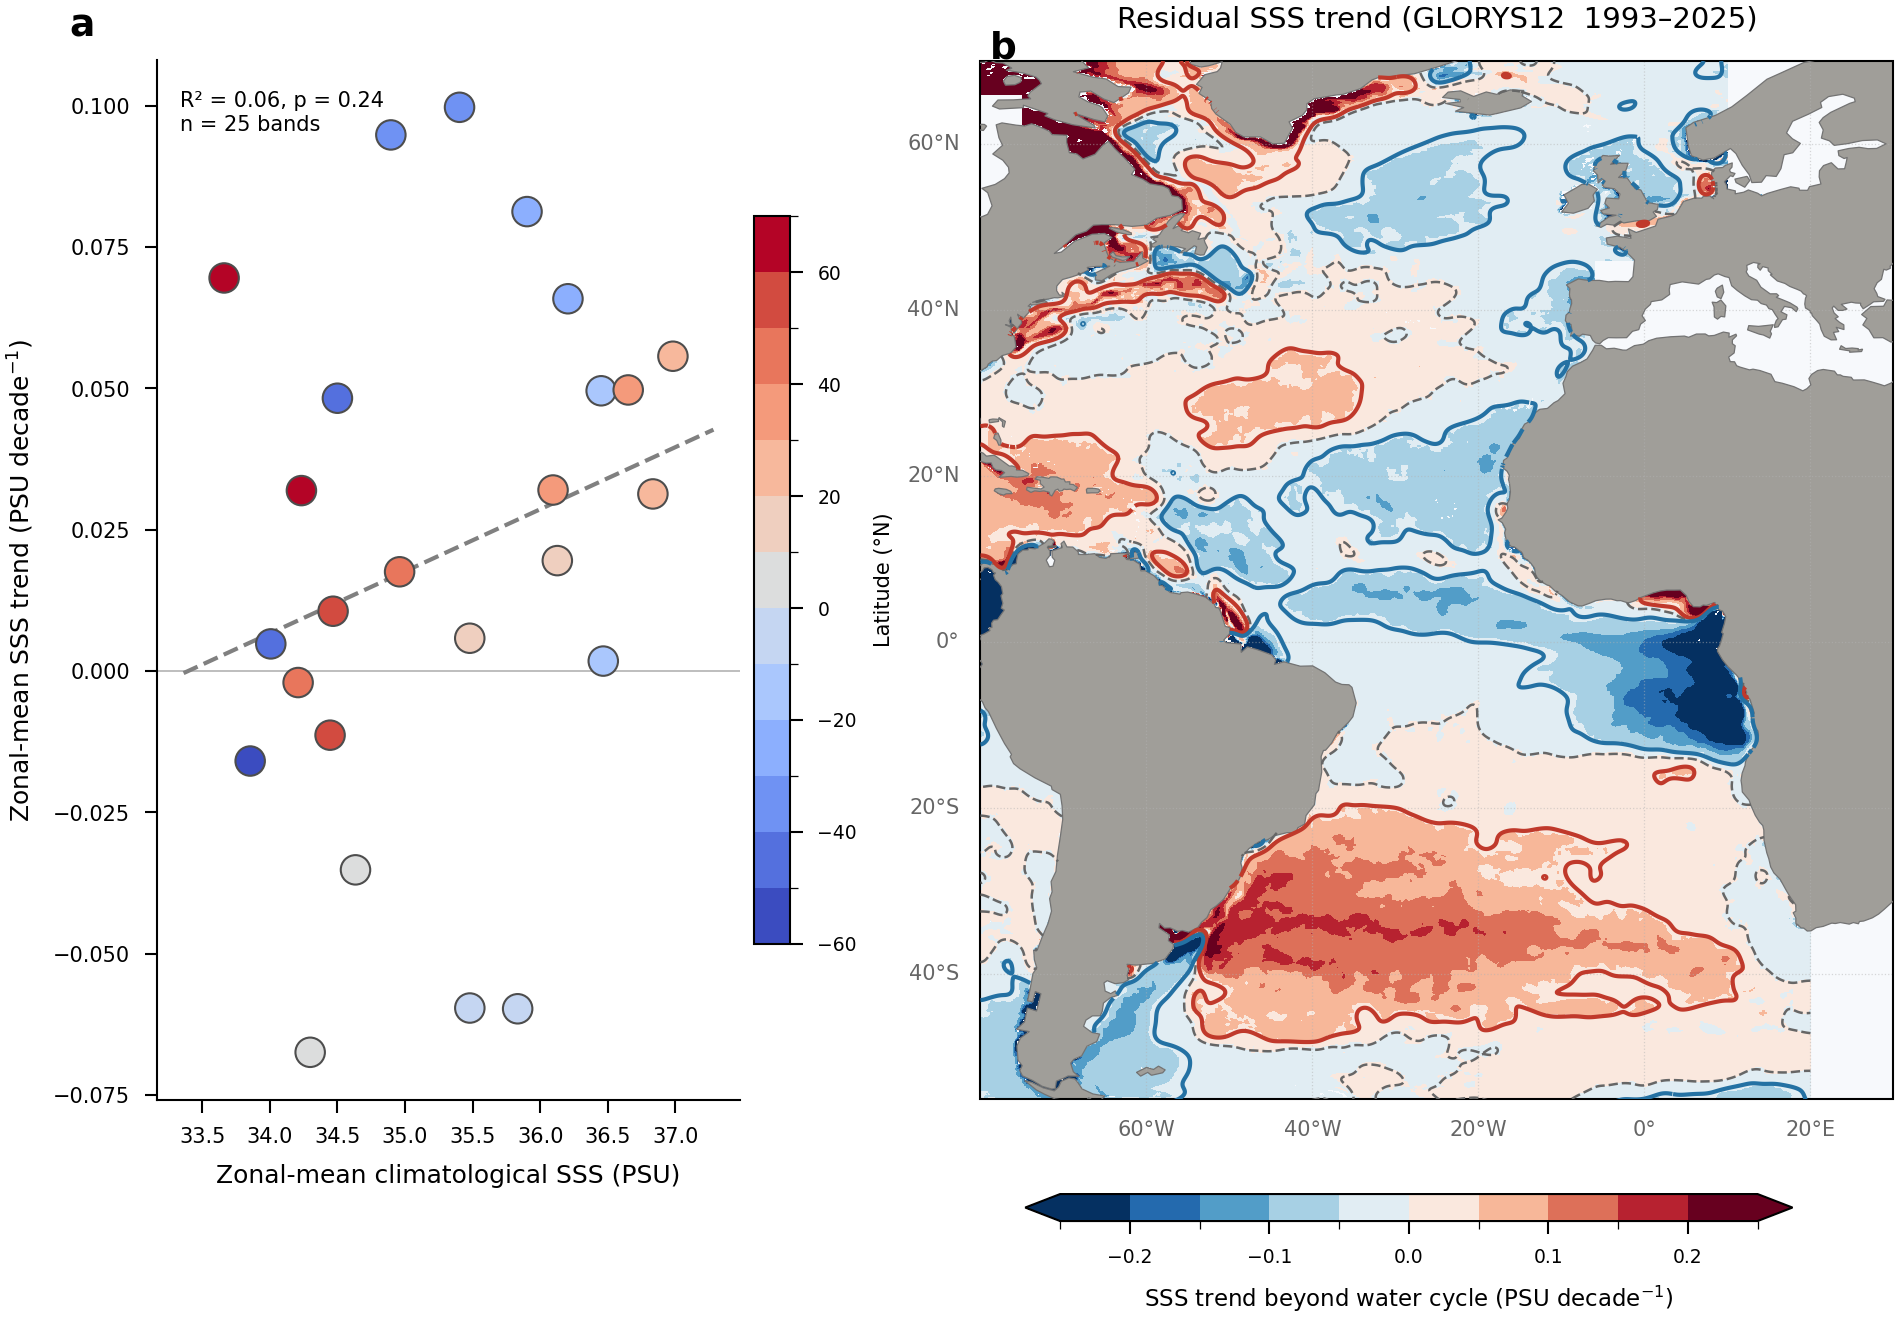
\includegraphics[width=\textwidth]{../figures/grl/fig_sss_decomposition.png}
\caption{Decomposition of Atlantic SSS trends into hydrological cycle and ocean dynamics components (GLORYS12V1, 1993--2025). Zonal-mean climatological SSS versus zonal-mean SSS trend across 25 latitude bands, colored by latitude. The dashed line shows the amplification regression ($R^2 = 0.06$, $p = 0.24$), which predicts that SSS trends should mirror the mean pattern under greenhouse-driven water cycle intensification. The weak relationship indicates that ocean dynamics, not the hydrological cycle, dominate Atlantic SSS trends.}
\label{fig:sss_decomp}
\end{figure}

\begin{figure}
\centering
\noindent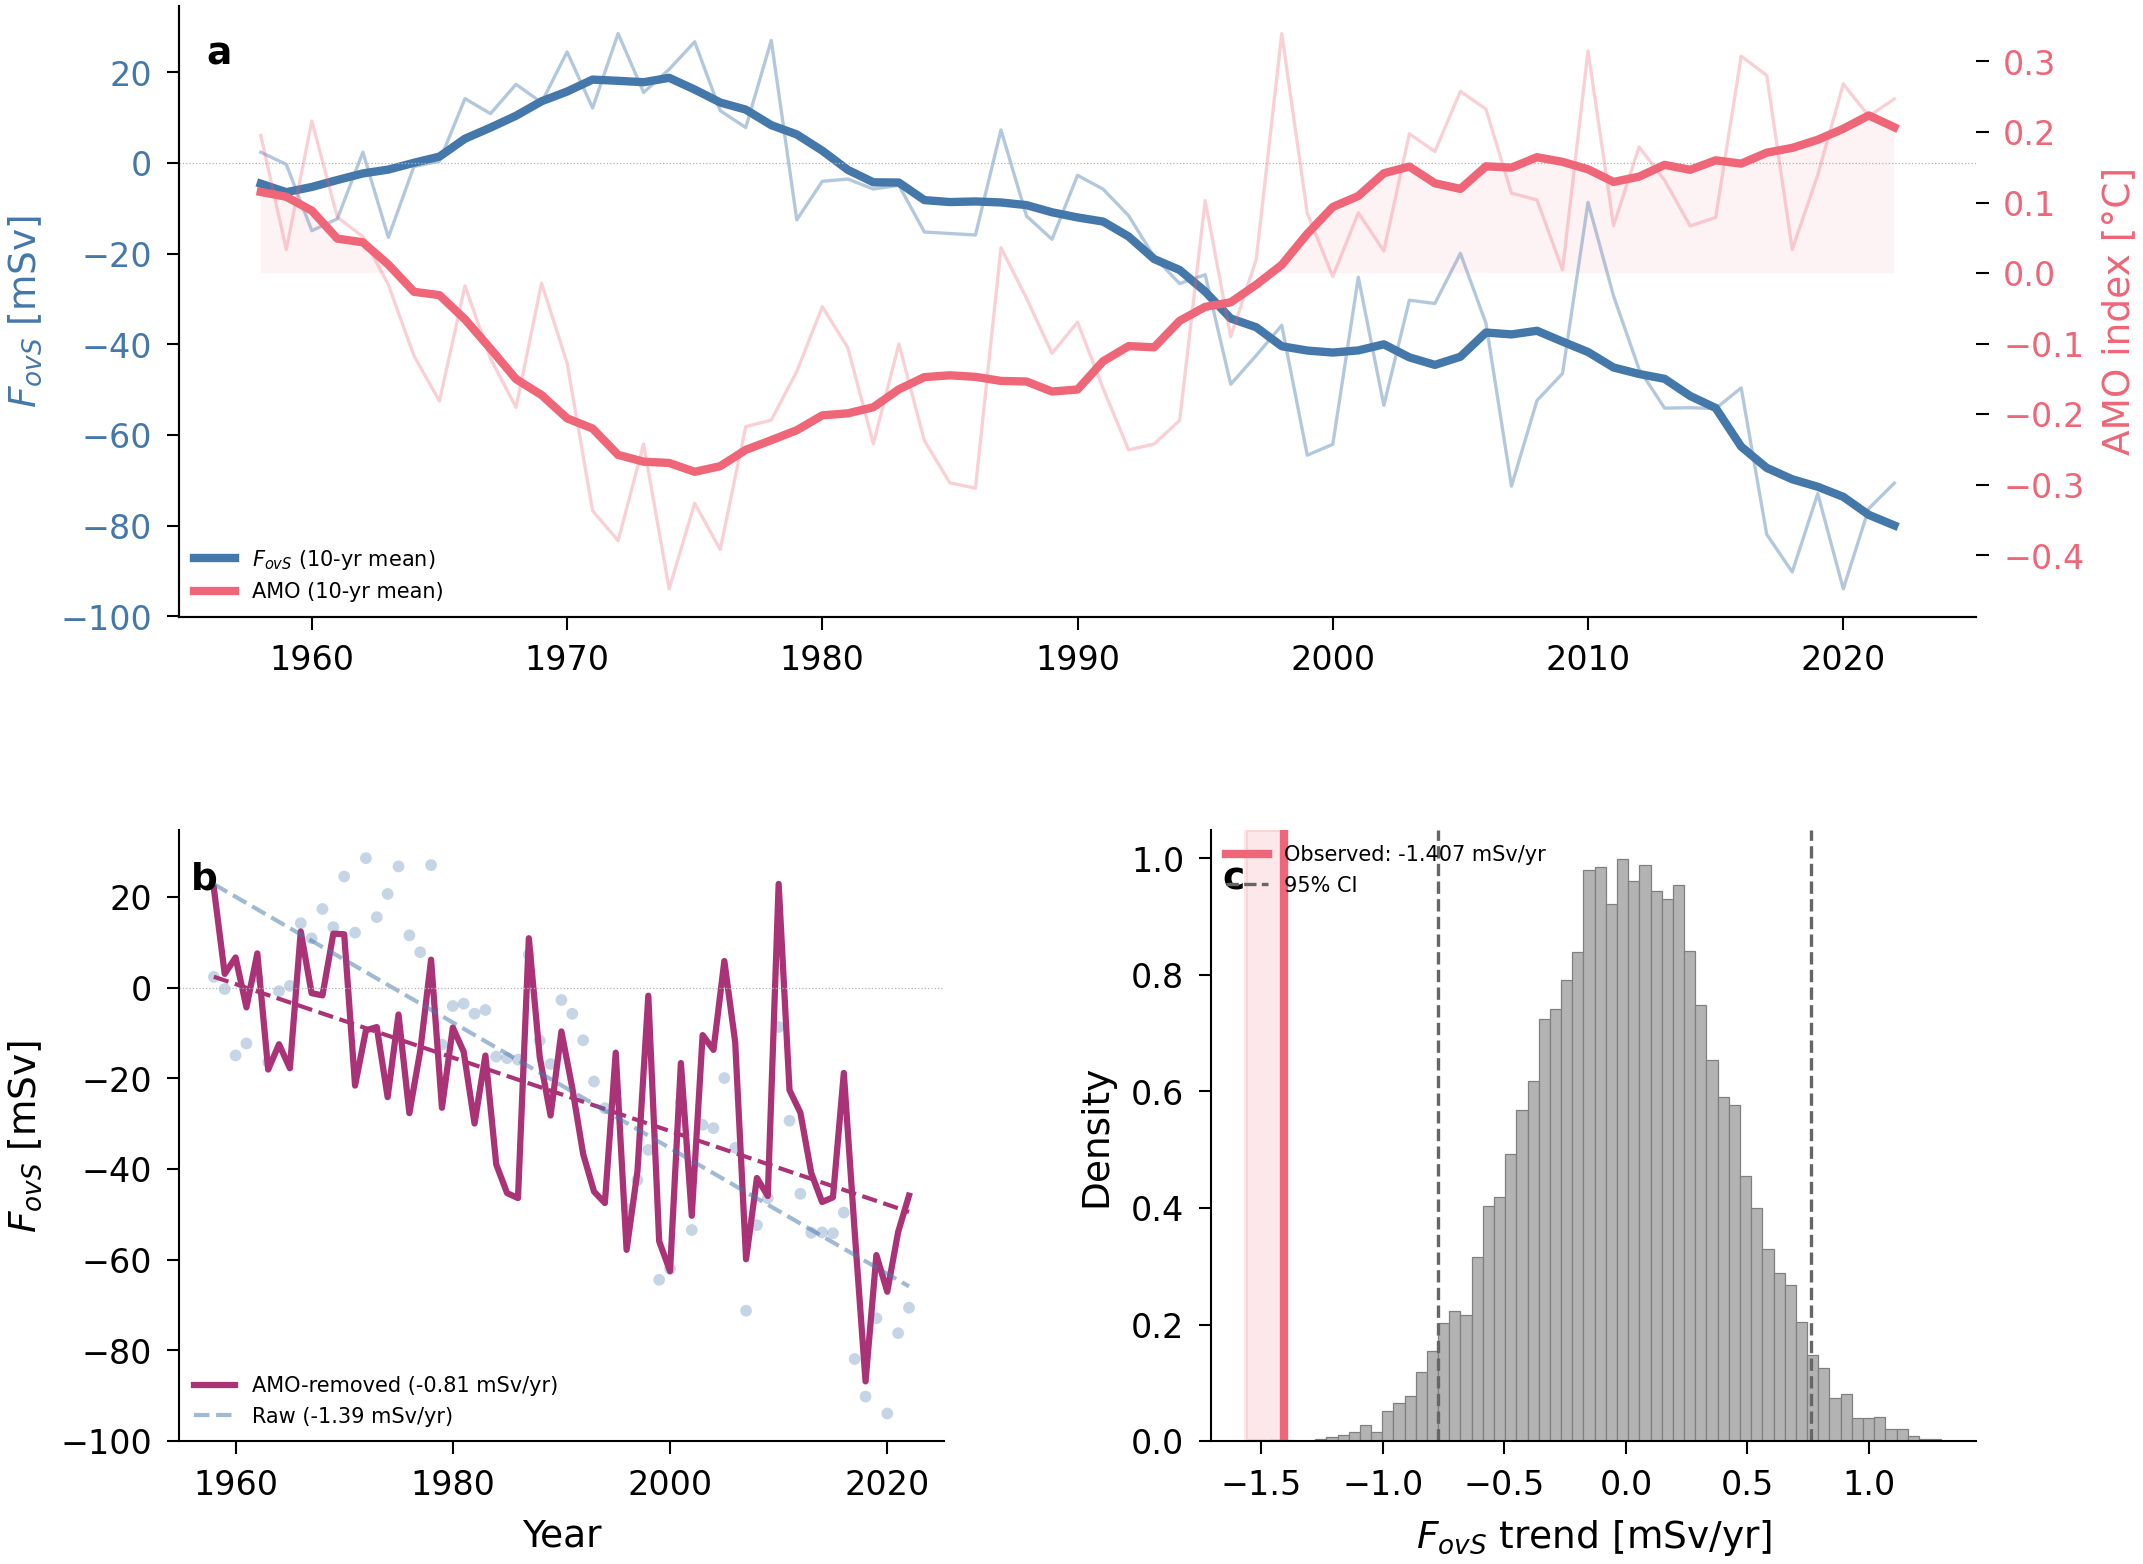
\includegraphics[width=\textwidth]{../figures/grl/fig_attribution.png}
\caption{Attribution of the F$_{ovS}$ decline. (a) Annual-mean F$_{ovS}$ (blue, left axis) and AMO index (red, right axis) with 10-year running means. Light red shading highlights the positive AMV phase (1998--present). Despite the AMO recovering to positive values, F$_{ovS}$ continues to decline, indicating decoupling from internal Atlantic variability. (b) F$_{ovS}$ after statistically removing the AMO-correlated component (purple). The residual trend ($-0.74$~mSv~yr$^{-1}$, $p < 10^{-7}$) represents 57\% of the raw trend. Raw annual values (grey dots) and raw trend (dashed blue) shown for comparison. (c) Block bootstrap null distribution (5-year blocks, 10,000 iterations) of the F$_{ovS}$ trend. The observed trend (red line, $-1.31$~mSv~yr$^{-1}$) falls outside the 99.99th percentile of the null distribution (dashed lines mark 95\% CI).}
\label{fig:attribution}
\end{figure}


\end{document}
